\section{Definition der Objekt-Struktur} \label{Objektstruktur}

	Wie bereits für die Skills wird auch für die Objekte eine Grundstruktur festgelegt, die als Basis für den Aufbau aller Objekte dient. Diese einheitliche Struktur erleichtert die Standardisierung der Interaktionen innerhalb der Software. Dabei sollen die Objektklassen möglichst objektorientiert gestaltet werden, sodass die Funktionalität der Objekte in klar abgegrenzten Methoden abgebildet wird. Zum Ausführen einer Funktionalität reicht es daher, die entsprechende Methode aufzurufen. 
	\\
	Die Objekte wurden zusammen mit dem Skills iterativ erarbeitet. Änderungen bei der Skill-Struktur hatten auch einen Einfluss auf die Objektstruktur. 
	\\
	Die Schnittstellen eines Objektes wurden in 4 Kategorien aufgeteilt, welche ähnlich wie beim Skill definiert wurden (siehe Kapitel \ref{Skillstruktur}) und entsprechend das allgemeine Verständnis einfacher machen sollen. 
	
	\textbf{Objektvariablen:}
	\vspace{2mm} 
	\\
	Die Objektvariablen umfassen die Eingangsvariablen (Objektparameter) und die Ausgangsvariablen (Anlagenparameter), welche für den Betrieb des Objektes benötigt werden. Dabei kann es sich z.B. um eine IP-Adresse handeln, wenn das Objekt über eine TCP/IP-Schnittstelle angesprochen wird. Falls das Objekt direkt mit E/A-Klemmen interagieren muss, kann dies über die Anlagenparameter gemacht werden. 
	
	
	\textbf{Steuerungselemente:}
	\vspace{2mm} 
	\\
	Die Steuerungselemente sind für die Bedienung des Objektes angedacht. Hier wird das Objekt gestartet, gestoppt oder resettet. Zusätzlich werden auch Informationen über den Zustand des Objektes angegeben.
	
	
	\textbf{Betriebselemente:}
	\vspace{2mm} 
	\\
	Die Betriebselemente sind für den allgemeinen Betrieb des Objekts angedacht, welche nicht mit dem spezifischen Prozess zu tun haben. Dies ist z.B. die Schnittstelle zum System, welche eine Aussage über Systemzustand macht.
	
	
	\textbf{Prozesselemente:}
	\vspace{2mm} 
	\\
	Die Prozesselemente sind spezifische Informationen, welche das Objekt für die Ausführung benötigt.
	
	Die Steuerungs-, Betriebs- und Prozesselemente erfüllen somit die gleichen Aufgaben wie beim Skill. Zwischen der Struktur von Objekten und Skills gibt es bewusste Parallelen, welche die Verständlichkeit und Übersicht der Gesamtsoftware verbessern sollen. Die Steuerungselemente umfassen die gleichen Methoden und Eigenschaften wie die Skills (Tab. \ref{tab:Objekt_Steuerungselemente}) (Umsetzung dieser unterscheidet sich jedoch). 
	
	\newcolumntype{L}[1]{>{\raggedright\let\newline\\\arraybackslash\hspace{0pt}}m{#1}}
	\begin{table}[ht]
		\centering
		\colorlet{BFH-table}{BFH-MediumBlue!10}
		\colorlet{BFH-tablehead}{BFH-MediumBlue!50}
		\begin{bfhTabular}{| l | l | L{3.7cm} | L{5cm} |}
			Art: 		& Bezeichnung:		& Typ:		& Beschreibung:								
			\\\hline
			Methode		& \verb|M_Start|	& \verb|BOOL|			& Methode zum Starten des Objektes
			\\\hline
			Methode		& \verb|M_Stop|		& \verb|BOOL|			& Methode zum Stoppen des Objektes
			\\\hline
			Methode		& \verb|M_Reset|	& \verb|BOOL|			& Methode zum Resetten des Objektes
			\\\hline
			Eigenschaft	& \verb|P_State|	& \verb|eObjectAktorState| / \verb|eObjectSensorState| & Eigenschaft des aktuellen Zustandes
		\end{bfhTabular}
		\captionsetup{justification=centering}
		\caption{Steuerungselemente eines Objektes}
		\label{tab:Objekt_Steuerungselemente}
	\end{table}
	
	Die Eigenschaft wird mit einem benutzerdefinierten \verb|ENUM|-Datentyp (Tab. \ref{tab:Datentypen_Benutzerdefiniert_Objekt}) umgesetzt, welcher die Zustände des Objektes abbildet. Somit ist immer klar, in welchem Zustand sich das Objekt im Moment befindet. Dabei unterscheidet man zwischen Aktor und Sensor. 
	
	\begin{table}[ht]
		\centering
		\colorlet{BFH-table}{BFH-MediumBlue!10}
		\colorlet{BFH-tablehead}{BFH-MediumBlue!50}
		\begin{bfhTabular}{ccc}
			Listen-Nr: 	& \verb|eObjectAktorState|:		& \verb|eObjectSensorState|:				
			\\\hline
			0			& \verb|AUS|					& \verb|AUS| 
			\\\hline
			1			& \verb|BEREIT|					& \verb|LAUFEND|
			\\\hline
			2			& \verb|MANUELL|				& \verb|FEHLER|
			\\\hline
			3			& \verb|LAUFEND|				& \verb|/|
			\\\hline
			4			& \verb|ABGESCHLOSSEN_INTERN|	& \verb|/|
			\\\hline
			5			& \verb|ABGESCHLOSSEN_EXTERN|	& \verb|/|
			\\\hline
			6			& \verb|GESTOPPT|				& \verb|/|
			\\\hline
			7			& \verb|FEHLER|					& \verb|/|
		\end{bfhTabular}
		\captionsetup{justification=centering}
		\caption{Benutzerdefinierte Objekt-Datentypen}
		\label{tab:Datentypen_Benutzerdefiniert_Objekt}
	\end{table}
	
	In Kapitel \ref{Softwareinteraktion} (Struktur) wurden die Zustände eines Objekts definiert. Dies stellte einen wichtigen Schritt dar, um die allgemeine Interaktion zwischen System, Skill und Objekt festzulegen. Basierend auf diesen Zuständen wurden die finalen Zustände eines Objekts spezifiziert (Abb. \ref{fig:Objektzustände}).
	\\
	Ein Aktor-Objekt erweitert diese Zustände um einen zusätzlichen Zustand für den manuellen Betrieb. Ein Sensor-Objekt hingegen kann  einfacher gestaltet werden: Sobald das System eingeschaltet wird, ist der Sensor aktiv. Dieser Zustand wird nur durch das Ausschalten des Systems oder das Auftreten eines Fehlers verlassen.
	
		\newpage
	
	\begin{figure}[h!]
		\centering
		\includegraphics[width=0.8\textwidth]{07_Anlagenmodell/Objektzustände}
		\captionsetup{justification=centering}
		\caption{Objektzustände}
		\label{fig:Objektzustände}
	\end{figure}
	
	Auch in der Struktur unterscheiden sich Aktor- und Sensor-Objekte geringfügig. Sensor-Objekte verfügen über keine Steuerungsmethoden wie Start, Stopp oder Reset. Stattdessen werden diese Funktionen vom System über die Betriebsvariablen gesteuert.
	Beide Objekt-Typen verwenden jedoch dieselben Betriebsvariablen:
	
	\begin{table}[ht]
		\centering
		\colorlet{BFH-table}{BFH-MediumBlue!10}
		\colorlet{BFH-tablehead}{BFH-MediumBlue!50}
		\begin{bfhTabular}{clcl}
			Art: 				& Bezeichnung:			& Typ:				& Beschreibung:								
			\\\hline
			Eingangsvariabel	& \verb|eSysCommand|	& \verb|eSystemCommand|	& Befehl von System zu Skill
			\\\hline
			Eingangsvariabel	& \verb|eSysState|		& \verb|eSystemStatus|		& Informationen über System 
			\\\hline
			Eingangsvariabel	& \verb|iMode|			& \verb|INT|			& Objektmodus (Manuell / Automatik)
			\\\hline
			Ausgangsvariabel	& \verb|iErrorID|		& \verb|INT|				& Information über Fehler
		\end{bfhTabular}
		\caption{Betriebselemente eines Objektes}
		\label{tab:Objekt_Betriebselemente}
	\end{table}
	
	Wie in Kapitel \ref{Skillstruktur} beschrieben, verfügt ein Objekt über ein Interface, das die Steuerungselemente und Prozesseigenschaften definiert. Dieses Interface hängt von den erforderlichen Prozessparametern bzw. Prozessinformationen ab, sowie ob es sich um einen Aktor oder einen Sensor handelt. Die Prozessinformationen umfassen beispielsweise Messwerte eines Sensors oder die aktuelle Position eines Roboters.
	\\
	Die Grundstruktur eines Objekts wird im folgenden Schema (Abb. \ref{fig:Objektübersicht}) dargestellt. Es zeigt übersichtlich, wie das Objekt über die verschiedenen Schnittstellen im System interagiert.
	
	\newpage
	
	\begin{figure}[h!]
		\centering
		\begin{subfigure}[b]{0.45\textwidth}
			\centering
			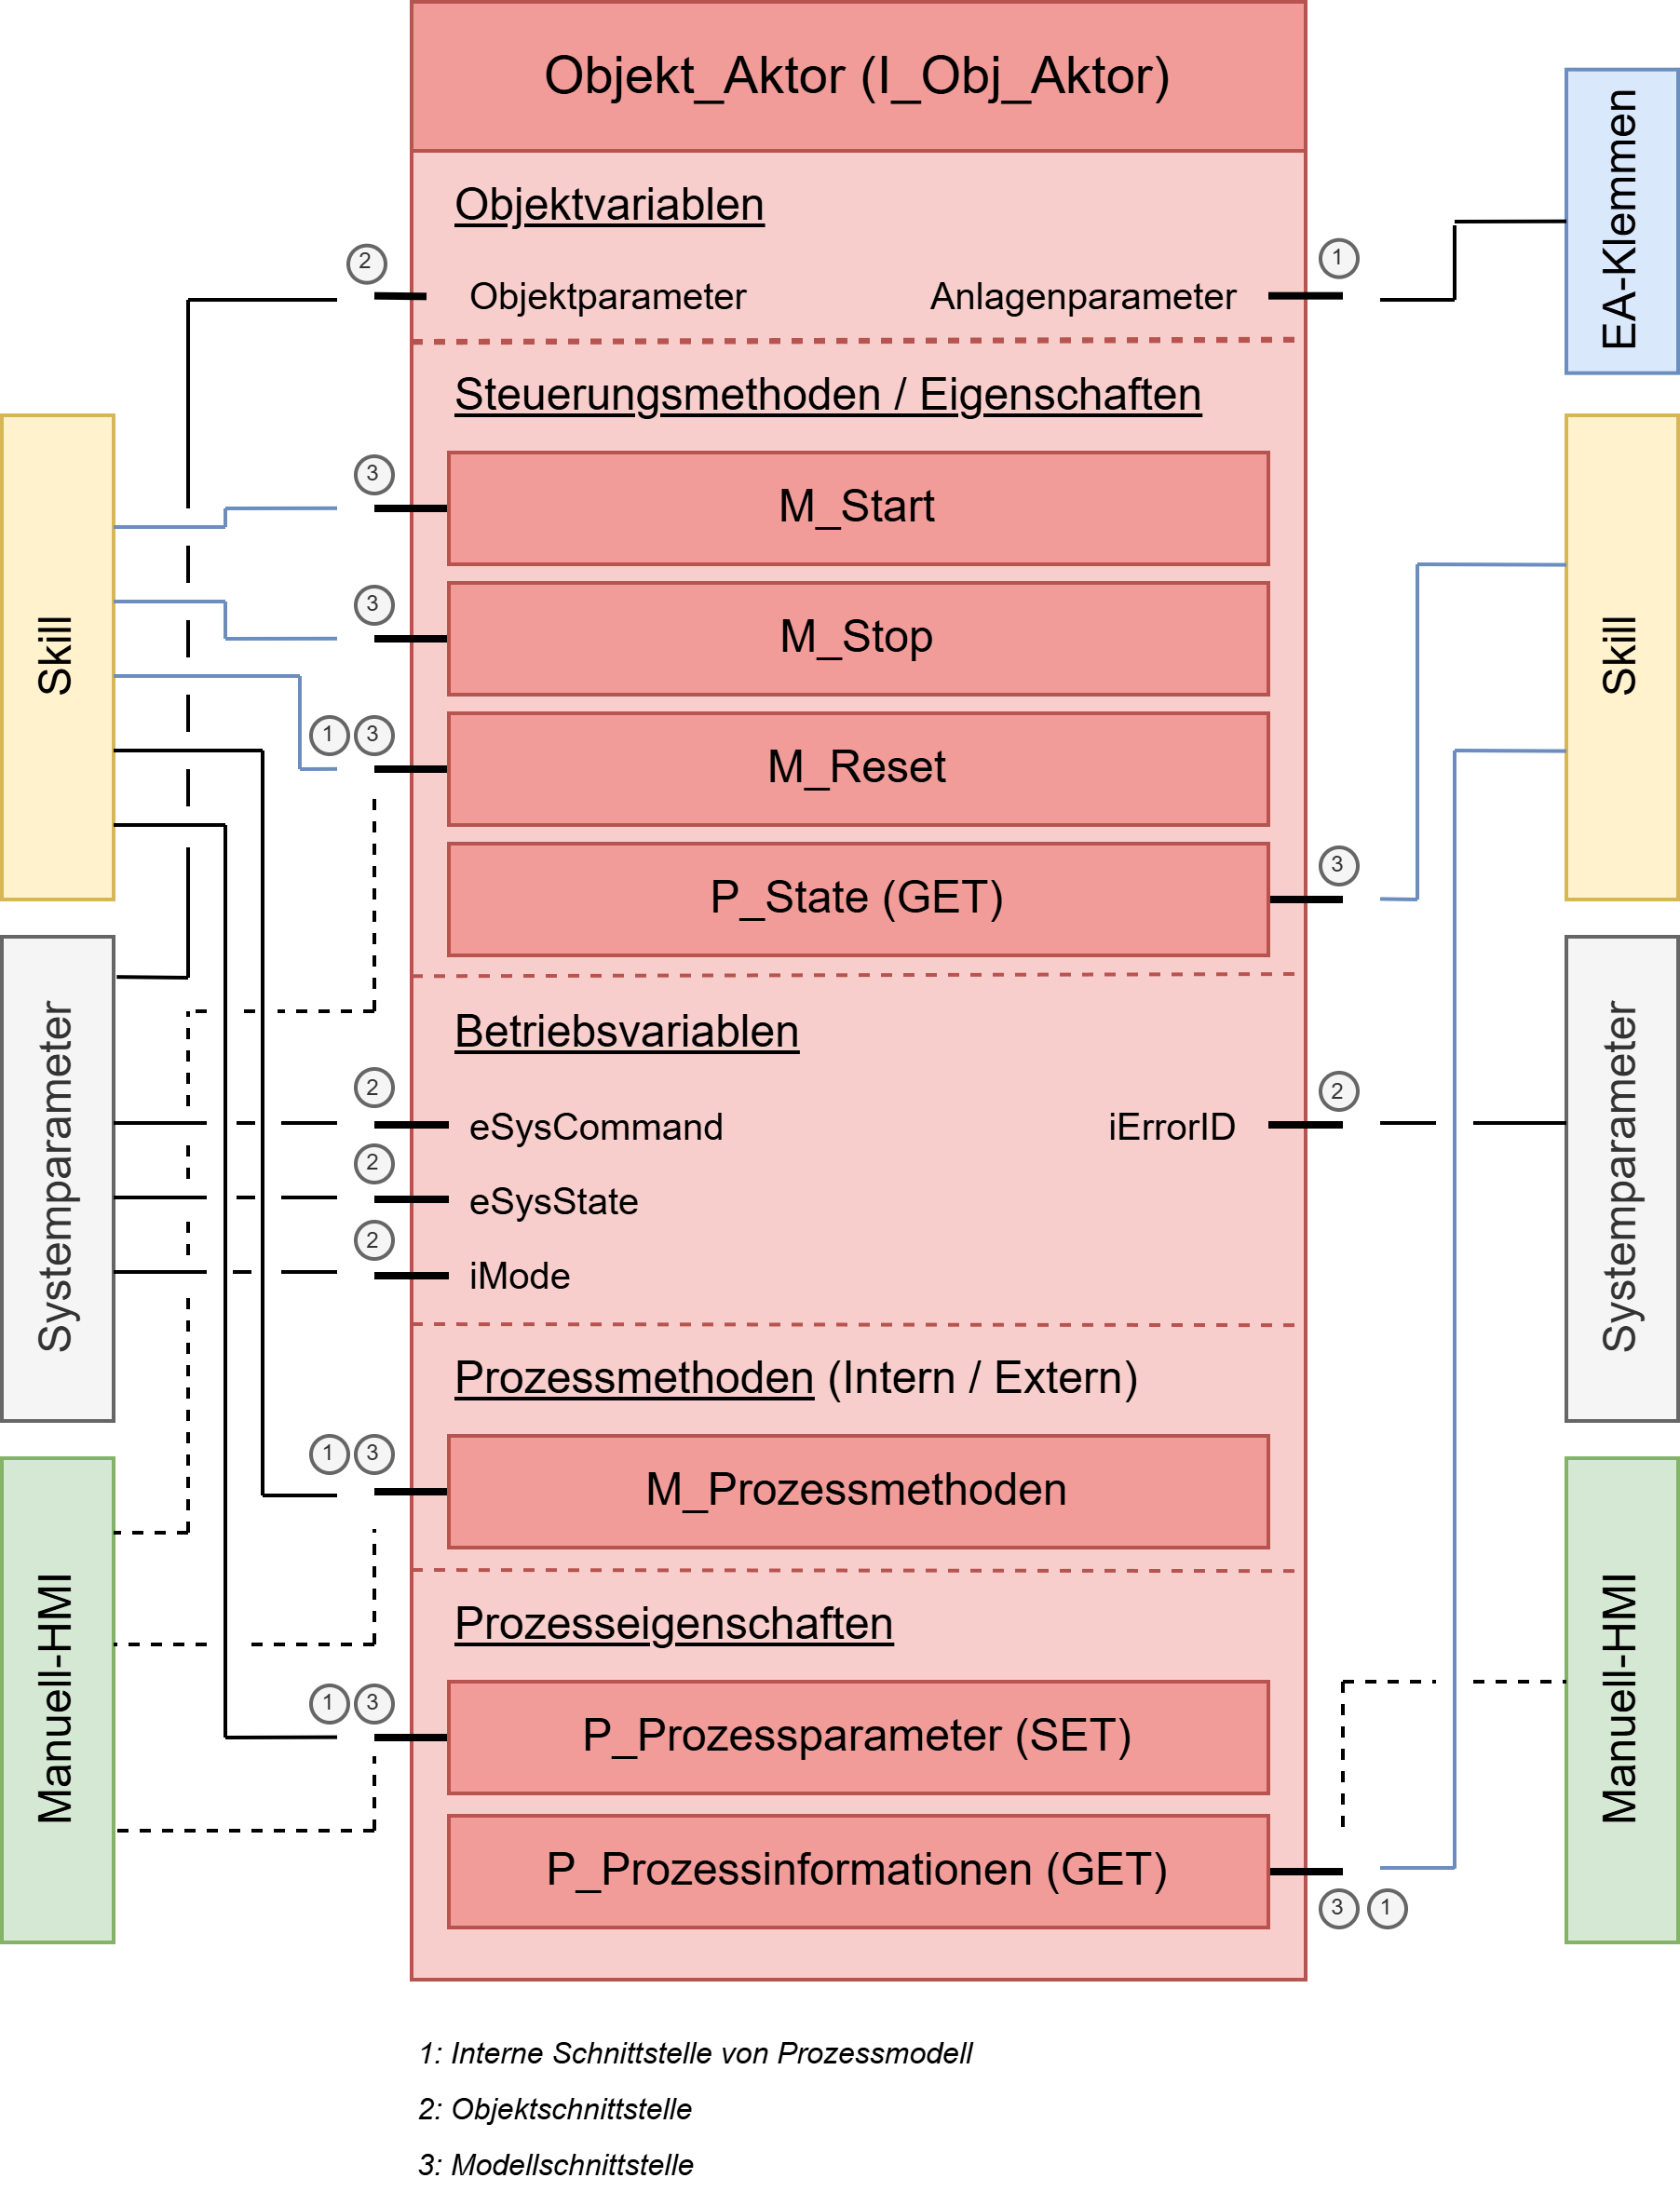
\includegraphics[width=\textwidth]{07_Anlagenmodell/AktorObjekt}
			\caption{Objektübersicht: Aktor}
			\label{fig:AktorObjekt}
		\end{subfigure}
		\hfill
		\begin{subfigure}[b]{0.45\textwidth}
			\centering
			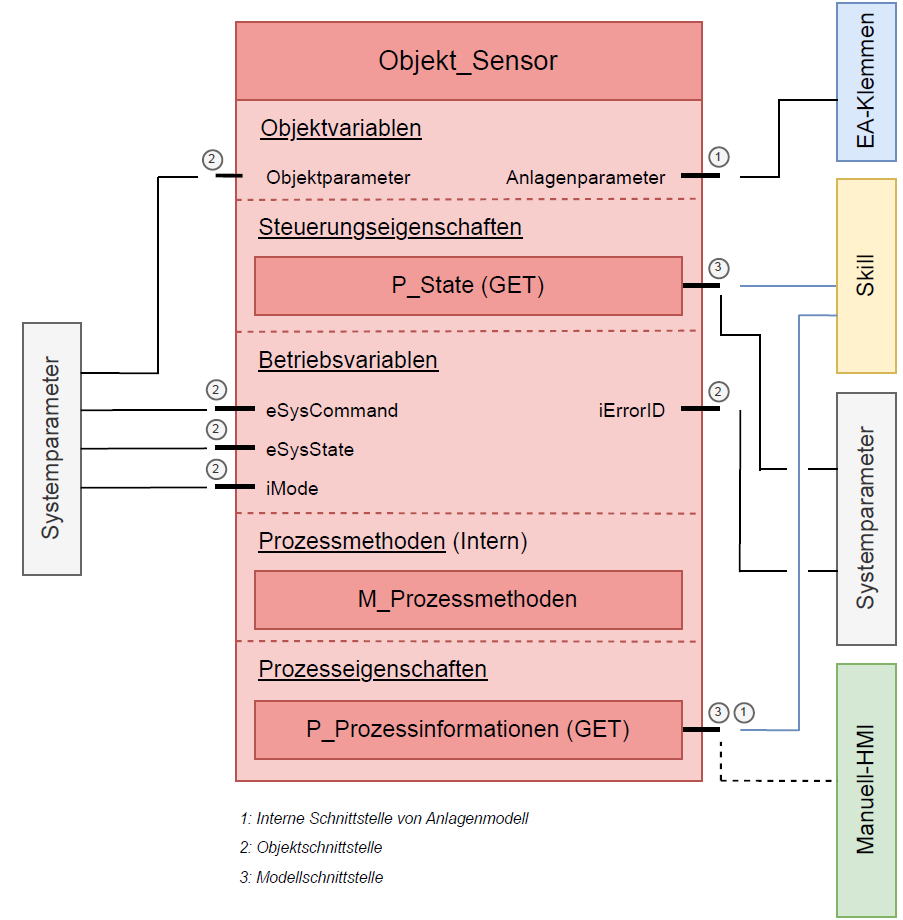
\includegraphics[width=\textwidth]{07_Anlagenmodell/SensorObjekt}
			\caption{Objektübersicht: Sensor}
			\label{fig:SensorObjekt}
		\end{subfigure}
		\caption{Objektübersicht}
		\label{fig:Objektübersicht}
	\end{figure}
	
	
	
	